\documentclass[reprint,amsmath,amssymb,aps,pra]{revtex4-2}

% ----------------------------------------------------------------------
% Packages

\usepackage{amsmath,amsthm,amssymb}

\usepackage{tikz}
\usetikzlibrary{calc, positioning, arrows}

\usepackage{hyperref}
\hypersetup{pdfencoding=unicode}

\usepackage{stmaryrd}
\usetikzlibrary{cd}
\usepackage[all,cmtip]{xypic}
\CompileMatrices

\usepackage{kbordermatrix}

% ----------------------------------------------------------------------
% For the bibliography

\newcommand{\arxiv}[1]{arXiv:\urlalt{https://arxiv.org/abs/#1}{#1}}

% ----------------------------------------------------------------------
% Theorem like environments

\theoremstyle{plain}
\newtheorem{theorem}{Theorem}[section]
\newtheorem{lemma}[theorem]{Lemma}
\newtheorem{corollary}[theorem]{Corollary}

\theoremstyle{definition}
\newtheorem{definition}[theorem]{Definition}
\newtheorem{remark}[theorem]{Remark}
\newtheorem{algorithm}[theorem]{Algorithm}

%----------------------------------------------------------------------
% A hack: \m is similar to \vcenter, but works better.
% \mp{0.2}{x}: raise the box x so that 20% of it is below the
% centerline. Unlike \vcenter, don't change the horizontal spacing

\newlength{\localh}
\newlength{\locald}
\newbox\mybox
\def\mp#1#2{\scalebox{0.8}{\setbox\mybox\hbox{#2}\localh\ht\mybox\locald\dp\mybox\addtolength{\localh}{-\locald}\raisebox{-#1\localh}{\box\mybox}}}
\def\m#1{\mp{0.4}{#1}}

%----------------------------------------------------------------------
% Ad hoc quantum circuits using TikZ

\newenvironment{qcircuit}{%
  \begingroup%
  \def\dot##1{\fill (##1) circle (.15);}%
  \def\whitedot##1{\filldraw[fill=white,thick] (##1) circle (.15);}%
  \def\triangle##1{\fill (##1)+(.3,0) --
    +(-.15,.25) -- +(-.15,-.25) -- cycle;}%
  \def\triangleadj##1{\fill (##1)+(-.3,0) --
    +(.15,.25) -- +(.15,-.25) -- cycle;}%
  \def\notgate##1{\filldraw[fill=white,thick] (##1) circle (.3);
                  \draw[thick] (##1)+(.3,0) -- +(-.3,0);
                  \draw[thick] (##1)+(0,.3) -- +(0,-.3);
                }%
  \def\dotgate{\dot}%
  \def\sepgate##1##2##3{
    \fill[fill=white] (##1-.05,##2-.4) rectangle (##1+.05,##2+.4);
    \fill[fill=white] (##1-.05,##3-.4) rectangle (##1+.05,##3+.4);
    \draw[thick, dashed] (##1,##2-.25) -- (##1,##3+.25);
  }%
  \def\swapgate##1##2##3{
    \fill[fill=white] (##1-.45,##2-.4) rectangle (##1+.45,##2+.4);
    \fill[fill=white] (##1-.45,##3-.4) rectangle (##1+.45,##3+.4);
    \draw[thick] (##1-.45,##2) -- (##1+.45,##3);
    \draw[thick] (##1-.45,##3) -- (##1+.45,##2);
  }%
  \def\controlledS##1##2{\controlled{\dotgate}{##1}{##2};%
    \path(##1) node[above right]{$i$}}%              
  \def\controlledSS##1##2{\controlled{\gate{$S$}}{##1}{##2}}%
  \def\controlledSSd##1##2{\controlled{\gate{$S^{\dagger}$}}{##1}{##2}}%
  \def\controlled{\gencontrolled{\dot}}%
  \def\whitecontrolled{\gencontrolled{\whitedot}}%
  \def\controlwires##1##2{\foreach\x in {##2} {
                    \draw[thick] (##1 |- 0,\x) -- (##1);
                  }}%
  \def\gencontrolled##1##2##3##4{\controlwires{##3}{##4};
                  ##2{##3};
                  \foreach\x in {##4} {
                    ##1{##3 |- 0,\x};
                  }}%
  \def\gate##1##2{\biggate{##1}{##2}{##2}}%
  \def\colgate##1##2##3{\widebigcolgate{##2}{##3}{##3}{.45}{##1}}%
  \def\colbiggate##1##2##3##4{\widebigcolgate{##2}{##3}{##4}{.45}{##1}}%
  \def\biggate##1##2##3{\widebiggate{##1}{##2}{##3}{.45}}%
  \def\widegate##1##2##3{\widebiggate{##1}{##3}{##3}{##2}}%
  \def\widebiggate##1##2##3##4{\widebigcolgate{##1}{##2}{##3}{##4}{white}}%
  \def\widecolgate##1##2##3##4{\widebigcolgate{##3}{##4}{##4}{##1}{##2}}%
  \def\widebigcolgate##1##2##3##4##5{\filldraw[fill=##5,thick] (##2)+(-1*##4,-.4)
    rectangle ($(##3)+(##4,.4)$); \draw ($.5*(##2)+.5*(##3)$) node
    {\small ##1};}%
  \def\invisiblewidebigcolgate##1##2##3{\path (##1)+(-1*##3,-.4)
    rectangle ($(##2)+(##3,.4)$);}%
  \def\invisiblegate##1{\invisiblewidebigcolgate{##1}{##1}{.45}}
  \def\gridx##1##2##3{\foreach\x in {##3} {
        \draw[thick] (##1,\x) -- (##2,\x);
      }}%
  \def\grid{\gridx{0}}%
  \def\cross##1{\draw (##1)+(-.3,-.3) -- +(.3,.3);
             \draw (##1)+(.3,-.3) -- +(-.3,.3);}%
  \def\bar##1{\fill (##1)+(-.05,-.4) rectangle ($(##1)+(.05,.4)$);}%
  \def\init##1##2{\bar{##2}; \leftlabel{##1}{##2};}%
  \def\term##1##2{\bar{##2}; \rightlabel{##1}{##2};}%
  \def\leftlabel##1##2{\draw (##2) node[left] {##1};}%
  \def\rightlabel##1##2{\draw (##2) node[right] {##1};}%
  \def\wirelabel##1##2{\draw (##2)+(0,-.15) node[above] {\footnotesize ##1};}%
  \def\multiwire##1{\draw (##1)+(-.1,-.3) -- +(.1,.3);}%
  \begin{tikzpicture}}
  {\end{tikzpicture}\endgroup}

%----------------------------------------------------------------------
% Alphabetic labels

{\makeatletter
\gdef\alphalabels{\def\theenumi{\@alph\c@enumi}\def\labelenumi{(\theenumi)}}}

% ----------------------------------------------------------------------
% Miscellaneous macros

\newcommand{\xmatrix}[4]{{\renewcommand{\arraystretch}{#1}\arraycolsep=#2ex\left(\begin{array}{#3}#4\end{array}\right)}}       % resizable matrix
\newcommand{\zmatrix}{\xmatrix{.8}{.8}}         % matrix
\newcommand{\smatrix}[1]{\begin{bmatrix} #1 \end{bmatrix}}         % matrix
\newcommand{\s}[1]{\left\{#1\right\}}
\newcommand{\cC}{{\cal C}}
\newcommand{\cT}{{\cal T}}
\newcommand{\cCS}{{\mathcal{CCS}}}
\newcommand{\Clifford}{\cC}
\newcommand{\CliffordCS}{\cCS}
\newcommand{\inv}{^{-1}}
\newcommand{\da}{^{\dagger}}
\newcommand{\CZ}{C\kern-.16667em Z}
\newcommand{\CX}{C\kern-.16667em X}
\newcommand{\CS}{C\kern-.16667em S}
\newcommand{\CK}{C\kern-.16667em K}
\newcommand{\XC}{X\kern-.16667em C}
\newcommand{\KC}{K\kern-.16667em C}
\newcommand{\Ex}{E\kern-.16667em x}
\newcommand{\LS}{L\kern-.16667em S}
\newcommand{\RS}{R\kern-.16667em S}
\newcommand{\CCZ}{CCZ}
\newcommand{\CCX}{CCX}
\newcommand{\CCK}{CCK'}
\newcommand{\Swap}{\textit{Swap}}
\newcommand{\CCS}{Clifford+$\CS$ }
\newcommand{\pres}[2]{\langle #1\mid #2 \rangle}


\newcommand{\Xx}{\mathcal{X}}
\newcommand{\Yy}{\mathcal{Y}}
\newcommand{\Rr}{\Delta}
\newcommand{\Ss}{\Gamma}
\newcommand{\Ee}{\mathcal{E}}

\newcommand{\Z}{\mathbb{Z}}
\newcommand{\jay}{j}
\newcommand{\kay}{k}
\newcommand{\tee}{t}
\newcommand{\svdots}{\scalebox{.55}{$\vdots$}}
\newcommand{\seq}{\subseteq}
\newcommand{\gen}[1]{\langle#1\rangle}
\newcommand{\sem}[1]{[#1]}
\newcommand{\semG}[1]{\sem{#1}_{G}}
\newcommand{\semH}[1]{\sem{#1}_{H}}
\newcommand{\simE}{\sim_{\Ee}}
\newcommand{\simR}{\sim_{\Rr}}
\newcommand{\simS}{\sim_{\Ss}}
\newcommand{\Ys}{Y_{s}}
\newcommand{\Rsyll}[1]{R_{#1}}
\newcommand{\ket}[1]{|#1\rangle}

\newcommand{\fst}[1]{\text{fst}(#1)}
\newcommand{\snd}[1]{\text{snd}(#1)}
\newcommand{\Zhi}{\Z[\frac{1}{2},i]}



\newcommand{\Mod}[1]{\,(\mathrm{mod}\ #1)}

\newcommand{\zi}{\Z [i]}
\newcommand{\di}{\D [i]}
\newcommand{\simr}{\sim_{\Rr}}
\newcommand{\oh}{K}
\newcommand{\lde}[1]{\text{lde}( #1 )}
\newcommand{\ldeg}[1]{\text{lde}_{\gamma}( #1 )}

\newcommand{\eqmo}{\equiv_{\gamma}}
\newcommand{\eqmt}{\equiv_{\gamma^2}}
\newcommand{\eqmth}{\equiv_{\gamma^3}}


\newcommand{\level}[1]{\text{level}(#1)}
\newcommand{\xal}{X_{[\alpha, \alpha+1]}}
\newcommand{\normalword}{\text{\rm normal}}
\newcommand{\nf}{\text{\sc nf}}

\newcommand{\tlx}[2]{X_{[#1, #2]}}
\newcommand{\tlkd}[2]{\oh^{\dagger}_{[#1, #2]}}
\newcommand{\tlk}[2]{\oh_{[#1, #2]}}
\newcommand{\tli}[2]{i_{[#1]}^{#2}}

\newcommand{\D}{{\mathbb D}}
\newcommand{\N}{{\mathbb N}}
\newcommand{\R}{{\mathbb R}}
\newcommand{\C}{{\mathbb C}}
\newcommand{\Gg}{\mathcal{G}}
\newcommand{\iso}{\cong}

\newcommand{\sfrac}[2]{{#1}/{#2}}   % short fraction
\newcommand{\norm}[1]{\|#1\|}


\newcommand{\eps}{\varepsilon}


\makeatletter
\newcommand{\xRightarrow}[2][]{\ext@arrow 0359\Rightarrowfill@{#1}{#2}}
\makeatother




% ----------------------------------------------------------------------
% Macros for large case distinctions

% \newcounter{case}
% \newcounter{subcase}[case]
% \newcounter{subsubcase}[subcase]
% \newcounter{subsubsubcase}[subsubcase]
% \newcounter{subsubsubsubcase}[subsubsubcase]

% \renewcommand{\thesubcase}{\thecase.\arabic{subcase}}
% \renewcommand{\thesubsubcase}{\thesubcase.\arabic{subsubcase}}
% \renewcommand{\thesubsubsubcase}{\thesubsubcase.\arabic{subsubsubcase}}
% \renewcommand{\thesubsubsubsubcase}{\thesubsubsubcase.\arabic{subsubsubsubcase}}

% \newcommand{\case}[1]{\refstepcounter{case}\par\noindent{\bf Case \thecase.} #1.}
% \newcommand{\subcase}[1]{\refstepcounter{subcase}\par\noindent{\bf Case \thesubcase.} #1.}
% \newcommand{\subsubcase}[1]{\refstepcounter{subsubcase}\par\noindent{\bf Case \thesubsubcase.} #1.}
% \newcommand{\subsubsubcase}[1]{\refstepcounter{subsubsubcase}\par\noindent{\bf Case \thesubsubsubcase.} #1.}
% \newcommand{\subsubsubsubcase}[1]{\refstepcounter{subsubsubsubcase}\par\noindent{\bf Case \thesubsubsubsubcase.} #1.}




\newcommand{\CliffordT}{\cC\cT}




\newcommand{\De}{\Delta}
\newcommand{\amal}{*}



%\newcommand{\sem}[1]{[#1]}

% Make sure this command does the same thing whether we use pdflatex
% or latex. The problem is that the \urlalt provided in some package
% (perhaps breakurl?) is different that the one provided by eptcs.
\providecommand{\urlalt}[2]{\href{#1}{#2}}
\renewcommand{\urlalt}[2]{\href{#1}{#2}}

\DeclareMathOperator{\rcs}{rcs}
\DeclareMathOperator{\cs}{cs}
\DeclareMathOperator{\kc}{kc}
\DeclareMathOperator{\rkc}{rkc}
\DeclareMathOperator{\rlen}{rlen}
\DeclareMathOperator{\len}{len}
\DeclareMathOperator{\pat}{pat}

\usepackage{svg}

\usepackage{pgfplots}
\pgfplotsset{compat=1.18}

\usepackage{breakurl}             % Not needed if you use pdflatex only.
% \usepackage{agda}

\usepackage{tkz-euclide}
\newenvironment{code}{%
  \begin{center}%
}{%
\end{center}%
}

\usepackage{algorithm}
\usepackage{algpseudocode}

\newcommand{\tab}{\hspace*{2em}}
\providecommand{\tabularnewline}{\\}

\usepackage{newunicodechar}
\newunicodechar{λ}{\ensuremath{\mathnormal\lambda}}
\newunicodechar{←}{\ensuremath{\mathnormal\from}}
\newunicodechar{→}{\ensuremath{\mathnormal\to}}
\newunicodechar{∀}{\ensuremath{\mathnormal\forall}}
\newunicodechar{ℕ}{\ensuremath{\mathbb N}}
\newunicodechar{≠}{\ensuremath{\mathnormal \neq}}
\newunicodechar{≡}{\ensuremath{\mathnormal \equiv}}
\newunicodechar{∈}{\ensuremath{\mathnormal \in}}
\newunicodechar{⊤}{\ensuremath{\mathnormal \top}}
\newunicodechar{⊥}{\ensuremath{\mathnormal \bot}}

\usepackage[normalem]{ulem}

\newcommand{\lb}{\bar{\lambda}}
\newcommand{\gb}{\bar{\gamma}}
\newcommand{\sH}{K}

\usepackage{tikzit}
\input{circuits.tikzstyles}


%----------------------------------------------------------------------
\begin{document}

\title{K-Optimal and CS-Near-Optimal Exact Synthesis of Two-Qubit
	Clifford+CS Operators}

\author{Xiaoning Bian} \email{bian@mail.tsinghua.edu.cn}

\author{Yuan Feng} \email{yuan\_feng@tsinghua.edu.cn}

\affiliation{Department of Computer Science and Technology, Tsinghua
	University}

\date{\today}

\begin{abstract}
  We present a method for decomposing a two-qubit Clifford+CS operator
  (equivalently, a $4\times 4$ unitary with entries in
  $\D[i] = \Z[\tfrac{1}{2}, i]$~\cite{Amy-Glaudell-Ross}) into a
  Clifford$+$CS circuit without ancillae. Let $k$ denote the least
  number of $K$ (scaled $H$) gates needed to implement a given unitary
  $U$. Our method decomposes $U$, up to a global phase, into a circuit
  of length at most $10k+9$, using exactly $k$ K gates and at most
  $k+1$ CS gates. The K-count is therefore optimal, and the CS-count
  is at most $2$ times optimal. We also improve the lower bound on the
  optimal CS-count from~\cite{Glaudell2021} by a factor of $2$. Let
  $l$ be the least natural number such that the entries of $(1+i)^l U$
  are all Gaussian integers; we prove that $k \in \{2l, 2l-1,
  2l-2\}$. In experiments, our method always achieves the optimal
  CS-count and reduces the $K$-count by 19\% on average relative to
  the best known prior algorithm. Part of our approach adapts the
  residue analysis of Russell~\cite{russell2014} for the Clifford$+T$
  gate set, with two main differences: we give explicit gate-count
  bounds (e.g., $10k+9$ rather than $O(k)$, where the two $k$'s are
  different but related), and we work over the simpler ring
  $\Z[\tfrac{1}{2}, i]$, a subring of the $\Z[\tfrac{1}{\sqrt 2}, i]$
  used by Russell.
\end{abstract}

\maketitle

\section{Introduction}

In quantum computation, decomposing unitary operators into gates from
a fixed universal set is a fundamental problem
\cite{Nielsen-Chuang}. The Clifford+Controlled-S gate set
(Clifford+CS) is universal, as is the well-studied Clifford+T gate
set. We study the exact synthesis of two-qubit Clifford+CS
operators. Prior work on two-qubit Clifford+CS and Clifford+T
synthesis has mainly aimed at minimizing the CS-count or T-count,
since these non-Clifford gates are typically the costliest
resource. However, work on T-gate optimization
\cite{Soken2014,AmyTOpt2014,Heyfron_2019,Kissinger2020,debeaudrap2020fast,de_Beaudrap_2020}
has identified the H gate as a bottleneck. As Soeken et
al.~\cite{Soken2014} put it: ``It has been shown that T-depth
optimizations can be implemented efficiently for circuits consisting
only of T and CNOT gates and that H gates impede the optimization
significantly.''


We propose a method that produces circuits with a minimal number of K
(scaled H) gates and a near-minimal number of CS gates, thereby
mitigating the H-gate bottleneck. Simultaneously minimizing two
distinct gate counts is also of mathematical interest. Earlier work on
single-qubit Clifford+T synthesis achieved the simultaneous minimum of
the Hadamard and T counts \cite{matsumoto2008,kliuchnikov2013fast,
  giles2013remarks}; extending this result to the multi-qubit case has
remained open.


\subsection{Background}
Consider the following unitary operators:
\begin{equation*}\label{eqn-generators}
  i,
  K = \omega^{7} H = \frac{1}{1+i}\begin{bmatrix}1&1\\1&-1\end{bmatrix},
  S = \smatrix{1&0\\0&i}, \text{ and}
\end{equation*}
\begin{equation*}
  \CZ =  \smatrix{1&0&0&0\\0&1&0&0\\0&0&1&0\\0&0&0&-1}.
\end{equation*}
Here, $i$ is the complex unit; $\omega = e^{\frac{i\pi}{4}}$ is a
primitive 8th root of unity; $H$ is the Hadamard gate and $K$ is a
scaled version of $H$; $S$ is sometimes called the \emph{phase gate};
and $\CZ$ is the controlled-$Z$ gate. Under multiplication,
identities, and tensor products, these operators generate the
\emph{Clifford group}. The precise group depends on which scalars are
included; we include only $\pm 1$ and $\pm i$, so the above gates
generate the Clifford group exactly.

Every operator $U$ obtained in this way is of size $2^n\times 2^n$ for
some $n \in \N$; we say that $U$ acts on $n$ qubits. For each $n$, the
group of $n$-qubit Clifford operators is finite (see, e.g.,
\cite{selinger2013generators}), so the Clifford gate set alone is not
universal for quantum computing. Universality is recovered by adding
the controlled phase gate
\begin{equation*}
  \CS = \smatrix{1&0&0&0\\0&1&0&0\\0&0&1&0\\0&0&0&i}.
\end{equation*}
The resulting operators are called Clifford+$\CS$ operators; note that
$\CZ = \CS^2$. We write $\CliffordCS$ for the group of two-qubit
Clifford+$\CS$ operators.

We adopt the following notational conventions. Single-qubit gates
lifted to two qubits are subscripted by the active qubit:
$K_0 = K \otimes I$, $K_1 = I \otimes K$, and likewise for $S_0$,
$S_1$, where $I$ is the $2 \times 2$ identity. The scalar $i$ is
identified with the $4\times 4$ matrix $i\,(I\otimes I)$. For
controlled gates, the last subscript denotes the target qubit; for
example, $\CX_{01}$ is the controlled-$X$ with control qubit $0$ and
target qubit $1$, abbreviated $\CX$, while $\CX_{10}$ is abbreviated
$\XC$. Since the controlled-$S$ and controlled-$Z$ gates are symmetric
($\CS_{jk}=\CS_{kj}$ and $\CZ_{jk}=\CZ_{kj}$), we simply write $\CS$
and $\CZ$.

We also use the $Z$- and $X$-gates, the controlled-$K$ gate
$\CK = I \oplus K$, and the swap gate $\Ex$. These can be expressed in
terms of the primitive gates by $Z = S^2$, $X = KZK \cdot i$,
$\CX = K_1\CZ K_1\cdot i$, $\Ex = \CX \, \XC \, \CX$, and
\begin{equation}
  \label{eqn:ck}
  \CK = \CZ \, Z_0S_0Z_1S_1K_1\CS K_1S_1\cdot i.
\end{equation}
Equation~\eqref{eqn:ck} shows that $\CK \in \CliffordCS$. As with
$\CX$, we shorten $\CK_{01}$ to $\CK$ and $\CK_{10}$ to $\KC$.

\begin{definition}[Two-qubit Clifford+$\CS$ circuit]
  \label{def:cir}
  Let
  \[
    \mathcal G =
    \s{X_j,Z_k,S_l,K_m,\CZ,\CS,\CX,\XC,\Ex},
  \]
  where $j,k,l,m \in \s{0,1}$. We call $\mathcal G$ the two-qubit
  Clifford+$\CS$ gate set, and a two-qubit Clifford+$\CS$ circuit a
  finite sequence of elements of $\mathcal G$. We write $\cCIR$ for
  the set of two-qubit Clifford+$\CS$ circuits.
\end{definition}

Each circuit $D \in \cCIR$ implements a unique operator
$\sem{D} \in \CliffordCS$, giving a matrix-semantics map
$\sem{\_} : \cCIR \to \CliffordCS$. We adopt the
``matrix-multiplication'' convention: the semantics map satisfies
$\sem{A \cdot B} = \sem{A} \cdot \sem{B}$, which is the reverse of the
usual quantum-circuit order. Here the first $\cdot$ denotes circuit
concatenation and the second matrix multiplication; either may be
omitted when context is clear.

\subsection{Related work}

Operator synthesis can be performed exactly or approximately. We
restrict attention to exact synthesis and review the most closely
related work below.

\subsubsection{Single-qubit and single-qudit}
For single-qubit Clifford+$T$ synthesis,
\cite{matsumoto2008,kliuchnikov2013fast,giles2013remarks} achieve the
simultaneous minimum use of both the Hadamard and $T$ gates. For the
single-qutrit case, \cite{Glaudell_2019,Prakash2018} achieve the
minimum $T$-count, and \cite{Amolak2020} addresses the general
single-qudit case. Forest et al.~\cite{Forest2015} generalize exact
synthesis from Clifford+$T$ to single-qubit Clifford-cyclotomic gate
sets, and Kliuchnikov and Yard~\cite{KliuchnikovYard2015} develop a
general algebraic framework for exact synthesis over number rings,
unifying several gate sets under one theory.

\subsubsection{Two-qubit}

Three works on two-qubit synthesis guarantee optimality of a
non-Clifford gate. Glaudell et al.~\cite{Glaudell2021} give a
CS-optimal synthesis of Clifford+CS operators, and Li et
al.~\cite{Li_2023_CT2} give a T-near-optimal synthesis of Clifford+T
operators with worst-case $T$-count at most 10 times optimal. Neither
considers $H$-count optimization, although the former implies an
$H$-count at most 2 times optimal. More recently, Glaudell et
al.~\cite{GlaudellJarret2026} gave a high-performance exact synthesis
framework for two-qubit Clifford+$T$ circuits that optimizes the
$T$-count exactly, using a meet-in-the-middle strategy with algebraic
canonicalization and lookup tables. All three works rely on the
exceptional isomorphism $SU(4) \cong \operatorname{Spin}(6)$. Our
work, by contrast, does not use this isomorphism; instead, we employ
a residue analysis similar to that of Russell~\cite{russell2014}, but
over the simpler ring
$\Z[\tfrac{1}{2}, i] \subset \Z[\tfrac{1}{\sqrt 2}, i]$. Given a
unitary $U$, Russell's method outputs a circuit of gate count
$O(k)$, where $k$ is the least natural number such that the entries
of $(1+\omega)^k U$ lie in $\Z[\omega]$.

\subsubsection{Multi-qubit and multi-qutrit}

Multi-qubit Clifford+$T$ synthesis was introduced by Giles and
Selinger~\cite{GilesSelinger2013}, whose algorithm has worst-case gate
count $O(3^{2^n} n k)$, later improved by
Kliuchnikov~\cite{kliuchnikov2013} to $O(4^n n k)$. Glaudell et
al.~\cite{Amy-Glaudell-Ross} gave exact multi-qubit synthesis for
several subclasses of Clifford+$T$ operators such as Toffoli+Hadamard
and Clifford+CS. In particular, they showed that $U$ is a two-qubit
Clifford+CS operator if and only if $U$ is a $4\times 4$ unitary with
entries in $\Z[\tfrac{1}{2}, i]$. Amy et al.~\cite{amy2023improved}
adapted the method of~\cite{kliuchnikov2013} to Toffoli+Hadamard
operators with a similar gate-count improvement. None of these
multi-qubit synthesis works consider $T$-count optimality. Kliuchnikov
and Sch\"onnenbeck~\cite{KliuchnikovSchonnenbeck2024} recently
developed an optimal-search algorithm for multi-qubit exact synthesis
using $A^*$ search; for two-qubit circuits, its runtime is
proportional to the $T$-count. Exact synthesis of multi-qubit
Clifford+Cyclotomic operators is treated
in~\cite{Glaudell2024a,Dinh_2025}, and the multi-qutrit case
in~\cite{Glaudell2024b,Amolak2024}. Beyond these,
\cite{glaudell-metaplectic} proves that qutrit metaplectic gates are a
subset of Clifford+T, and~\cite{Mukhopadhyay2024b} proposes a
heuristic algorithm achieving $V$-gate optimality.

% ----------------------------------------------------------------------
\section{Some algebra}
\label{sec:algebra}

Before describing the synthesis algorithm, we develop the algebraic
groundwork on which it rests. The relevant rings are $\zi$ and $\di$,
together with the quotients $\zi/(\gamma^n)$, which provide a
fine-grained way to track how operators act on entries.

\subsection{Rings}

We write $\N=\s{0,1,\ldots}$ for the natural numbers and $\Z$, $\R$,
$\C$ for the integers, reals, and complex numbers, respectively. The
complex conjugate of $z \in \C$ is denoted $z^{\dagger}$. Let
$\Z[i]=\s{a+bi\mid a,b\in\Z}$ be the ring of Gaussian integers. As a
Euclidean domain~\cite{Bian_ED}, $\zi$ supports division with
remainder, greatest common divisors, divisibility, and primes
(non-units not expressible as products of two non-units). The element
$\gamma = 1+i$ is a Gaussian prime~\cite{ant-book}, and since
$\gamma^2 = 2i$, the elements $\gamma^2$ and $2$ are associates.
Using Euclidean division, one can verify that
\[
  \zi/(\gamma) = \{0,1\},\quad \zi /(2) = \zi/(\gamma^2) = \{0,1,i,
  1+i\},\quad
\]
\[
  \text{and}\quad \zi /(\gamma^3) = \{\pm 1,\pm i, 0, 1+i, 1- i, 2\}.
\]
(Strictly, $\zi/(\gamma)$ denotes the quotient ring of $\zi$ modulo
the ideal $(\gamma)$; the sets above list complete systems of residue
class representatives, with the implicit $\bmod\,(\gamma^n)$ omitted
for brevity.)

Let $\D=\Z[\tfrac{1}{2}]=\s{\tfrac{a}{2^k}\mid a\in\Z, k\in\N}$ be the
ring of \emph{dyadic fractions}, i.e., fractions whose denominator is
a power of~$2$. Consider the ring
$\D[i] = \s{r+si \mid r, s \in \D} = \Z[\tfrac{1}{2},i]$. For every
$t \in \di$, there exists some $k \in \N$ with $\gamma^k t \in \zi$,
motivating the following definition.

\begin{definition}
  Let $t \in \di$. A natural number $k$ is a \emph{denominator
    exponent} for $t$ if $\gamma^k t \in \zi$, equivalently, if
  $t = s/\gamma^k$ for some $s \in \zi$. The smallest such $k$ is the
  \emph{least denominator exponent} of $t$, denoted $\lde(t)$.

  We extend this notion to vectors and matrices: $k$ is a denominator
  exponent for a vector or matrix if it is a denominator exponent for
  all of its entries, and the lde of a vector or matrix is the least
  such $k$.
\end{definition}

\begin{remark}
  By direct enumeration, the lde of any two-qubit Clifford operator is
  at most $2$.
\end{remark}

\subsection{Residue rings}

The quotient ring admits the following well-known characterization:
\[
  \zi/(\gamma ^ n) = \left\{\sum_{i=0}^{n-1} b_i \gamma^i \text{ mod }
    (\gamma^n) \,|\, b_i \in \s{0,1} \right \}.
\]

We give an elementary proof by induction on $n$; a similar argument
for the case $\Z[\sqrt 2]/(\sqrt 2 ^ n)$ appears in
Clement~\cite{Clement_pri}. The base case $n=1$ is immediate. Assume
the claim for $n$: every $x \in \zi$ has the form
\[
  x = \sum_{i=0}^{n-1} b_i \gamma^i + k \gamma^n \text{ for some } k
  \in \zi.
\]
Writing $k = b_n + k'\gamma$ with $b_n \in \s{0,1}$ and substituting
yields
\[
  x = \sum_{i=0}^{n} b_i \gamma^i + k' \gamma^{n+1}, \quad \text{i.e.,
  } x \equiv \sum_{i=0}^{n} b_i \gamma^i \text{ mod } (\gamma^{n+1}).
\]
For brevity, we omit $\bmod\,(\gamma^n)$ when context is clear, and we
write the binary string $(b_0 b_1 \dots)_2$ for the sum; the
parentheses and subscript may be dropped when context makes the
binary-residue interpretation unambiguous.

Moreover, distinct binary strings yield distinct residue classes:
suppose $\sum_{i=0}^{n-1} b_i \gamma^i \equiv \sum_{i=0}^{n-1} b'_i
\gamma^i \pmod{\gamma^n}$, i.e., $\sum_{i=0}^{n-1} (b_i - b'_i)
\gamma^i = k\gamma^n$ for some $k \in \zi$. Reducing modulo
$(\gamma)$ gives $b_0 = b'_0$. After cancelling $b_0 - b'_0 = 0$ and
dividing through by $\gamma$, we obtain
\[
  \sum_{i=1}^{n-1} (b_i - b'_i) \gamma^{i-1} = k\gamma^{n-1},
\]
and reducing modulo $(\gamma)$ again gives $b_1 = b'_1$. Iterating
shows $b_i = b'_i$ for all $i$.

Let $\rho_n(x)$ denote the canonical projection from $\zi$ to its
$n$-digit residue. The proof above shows that $\rho_n$ is
\emph{stable} under increase of $n$: the first $n$ digits of
$\rho_{n+1}(x)$ coincide with $\rho_n(x)$. Moreover, $\rho_2$ is
stable under complex conjugation: $\rho_2(x^{\dagger}) =
\rho_2(x)$. We use $x \equiv_{\gamma^n} y$ as shorthand for
$x \equiv y \pmod{\gamma^n}$. Modulo $\gamma^3$, we have
\[
  \begin{array}{c|c|c|c|c|c|c|c}
    x & \rho_3(x) & x   & \rho_3(x) & x   & \rho_3(x) & x  & \rho_3(x) \\
    \hline
    1 & 100       & -1  & 101       & i   & 111       & -i & 110       \\
    0 & 000       & 1+i & 010       & 1-i & 011       & 2  & 001
  \end{array}
\]

The $\Mod{\gamma ^ n}$ residue classes form a commutative ring. Modulo
$\gamma^2$, the ring addition coincides with bitwise exclusive or
(denoted $\oplus$); $(10)_2$ is the multiplicative identity; $(00)_2$
is the zero element; and multiplication by $(01)_2$ is the right shift
operation. By distributivity,
$11 \cdot b_0b_1 = 10 \cdot b_0b_1 + 01 \cdot b_0b_1 = b_0(b_1\oplus
b_0)$. The additive inverse of an element is itself. Since
$\rho_{2}(i) = 11$, whenever $\rho_1(x)=1$, either $\rho_2(x) = 10$ or
$\rho_2(ix) = 10$. Similarly, modulo $\gamma^3$, the addition rule is
\[
  b_0b_1b_2 + b'_0b'_1b'_2 = (b_0\oplus b'_0)(b_1\oplus
  b'_1)(b_2\oplus b'_2 \oplus (b_0 \cdot b'_0)),
\]
where $\cdot$ denotes multiplication in $\Z[i]/({\gamma})$,
equivalently the logical ``and'' of two bits. The multiplicative
identity is $100$ and the zero element is $000$. Multiplication by
$010$ is a right shift by $1$ digit and multiplication by $001$ is a
right shift by $2$ digits. The rest of the multiplication table
follows by distributivity. The additive inverse is
\[
  -(b_0b_1b_2) = b_0b_1(b_2\oplus b_0).
\]
From the $\rho_3$ table, $\rho_3$ is not stable under complex
conjugation: if $\rho_3(x) = abc$, then
$\rho_3(x^{\dagger}) = ab(c \oplus b)$. Since $\rho_3(i) = 111$,
whenever $\rho_1(x) = 1$ there exists $k \in \s{0,1,2,3}$ with
$\rho_3(i^k x) = 100$.

\begin{definition}
  Let $l$ be a denominator exponent for $x \in \di$ (not required to
  be the least). The \emph{$(n,l)$-residue} of $x$ is
  $\rho_n^l(x) := \rho_n(\gamma^l x)$. For a vector or matrix $A$,
  $\rho_n^l(A)$ is defined entry-wise whenever $l$ is a denominator
  exponent for $A$.
\end{definition}


\begin{definition}
  For $x \in \Z[i]$, if $\rho_1(x) = 0$, we say $x$ is \emph{even},
  otherwise \emph{odd}.
\end{definition}

For example, $1+2i$ is odd, while $1+3i$ is even. In our convention,
an \emph{even} Gaussian integer is one divisible by $\gamma$ — not
necessarily by $2$. For ordinary integers $x \in \Z$, however,
evenness as an integer coincides with evenness as a Gaussian integer,
so our definition extends the standard notion of parity. The
following lemmas are straightforward.

\begin{lemma}
  \label{lem:parity-dagger-norm}
  Let $\alpha =a+bi \in \zi$. Then $\alpha$ is odd if and only if
  $\norm{\alpha}^2=a^2+b^2$ is an odd integer.
\end{lemma}

\begin{lemma}
  \label{lem:cancel-gamma}
  If $\alpha,\beta \in \zi$ satisfy
  $\alpha \gamma \equiv_{\gamma^{n+1}} \beta \gamma$, then
  $\alpha \equiv_{\gamma^n} \beta$.
\end{lemma}

\begin{lemma}
  \label{lem:k-odd}
  For $t\in \di$, if $k = \lde(t)>0$, then $\gamma^kt$ is odd.
\end{lemma}

\begin{lemma}
  \label{lem:add}
  The lde function on $\di$ and matrices with $\di$ entries is
  subadditive: for $x, y \in \di$ and matrices $A, B$ with $\di$
  entries,
  \[
    \lde(xy) \le \lde(x) + \lde(y), \, \lde(AB) \le \lde(A) + \lde(B).
  \] If $x, y$ are both odd, then equality holds.
\end{lemma}

\subsection{Action on residues}

We now describe how the basic operations — multiplication by $i$,
shifts, addition, subtraction, and the $K$ gate — act at the level of
residues. These computations underpin the case analysis in
Section~\ref{ssec:synthesis}.

If $\rho_2(x) = b_0b_1$, then $\rho_2(ix) = b_0(b_1 \oplus b_0)$; we
say $i$ \emph{acts} on $b_0b_1$ by sending it to
$b_0(b_1 \oplus b_0)$. Given an $n$-digit residue
$b_0 b_1 \ldots b_{n-1}$, a \emph{right shift} produces the
$(n{+}1)$-digit residue $0 b_0 b_1 \ldots b_{n-1}$; given an
$(n{+}1)$-digit residue $0 b_0 b_1 \ldots b_{n-1}$, a \emph{left
  shift} produces $b_0 b_1 \ldots b_n$. We only consider shifts that
are \emph{well-defined}: no information is lost and no unknown digits
are introduced. (The usual right-shift was used when describing
multiplication in $\zi/(\gamma^2)$ and $\zi/(\gamma^3)$.)  We write
$\RS(x)$ for the right shift of $x$ and $\LS(x)$ for the left shift.

\begin{lemma}
  \label{lem:right-shift}
  For $t\in \di$, $l$ a denominator exponent of $t$, we have
  \[
    \rho_{n+1}^{l+1}(t) = \rho_{n+1}^{l}(\gamma t) =
    \RS(\rho_n^{l}(t)),
  \]
  and if $\gamma ^ l t$ is even and $l>0$,
  \[
    \rho_{n}^{l-1}(t) = \rho_{n}^{l}(t/\gamma) =
    \LS(\rho_{n+1}^{l}(t)).
  \]
\end{lemma}

Let $x, y \in \D[i]$ have lde $l > 0$, so $\rho_2^l(x) = 1b$ and
$\rho_2^l(y) = 1b'$ for some $b, b' \in \s{0,1}$. Then
\[ \rho_2^l(x + y) = 1b + 1b' = 0(b \oplus b'), \] and applying a left
shift gives $\rho_1^{l-1}(x+y) = b \oplus b'$. The case of $x - y$ is
analogous, since subtraction in $\Z/(2)$ coincides with $\oplus$
(every element is its own additive inverse). Consequently, if
$b \oplus b' = 1$ then $\lde(x \pm y)$ decreases by $1$, and if
$b \oplus b' = 0$ with $l \ge 2$, then $\lde(x \pm y)$ decreases by at
least $2$.

Now suppose further that $\rho_3^l(x) = 10b$ and $\rho_3^l(y) = 10b'$.
Since dividing by $\gamma$ increases the lde by $1$, we obtain

\begin{align*}
  \rho_2^l(K \begin{bmatrix}
    x \\
    y
  \end{bmatrix})
  =
  \rho_2^l(\begin{bmatrix}
    (x+y)/{\gamma} \\
    (x-y)/{\gamma}
  \end{bmatrix})
  =
  \LS(\rho_3^l(\begin{bmatrix}
    x+y \\
    x-y
  \end{bmatrix})) \\
  =
  \begin{bmatrix}
    0(b \oplus b' \oplus 1) \\
    0(b \oplus b')
  \end{bmatrix}.
\end{align*}

Hence $\lde(K
\begin{bmatrix}
  x \\
  y
\end{bmatrix}) = l-1$, with one entry having lde $l-1$ and the other
at most $l-2$ (provided $l\ge 2$).

\begin{remark}
  \label{rmk:dec1}
  The $K$ gate, acting on a pair of entries with the same lde $l > 0$
  and proper residues, decreases the lde of the pair by at most
  $1$. Moreover, $K$ is the only gate in the Clifford+CS gate set that
  affects the lde at all. These two facts are needed for the
  optimality proof.
\end{remark}

In general, suppose $x, y \in \D[i]$ have lde $l > 0$. If
$\rho_3^l(x) = 1b_0 b_1$ and $\rho_3^l(y) = 1b'_0 b'_1$, then
\begin{align*}
  \rho_2^l(K \begin{bmatrix}
    x \\
    y
  \end{bmatrix})
  =
  \begin{bmatrix}
    (b_0\oplus b_0')(b_1 \oplus b_1' \oplus 1) \\
    (b_0\oplus b_0')(b_1 \oplus b_1')
  \end{bmatrix}.
\end{align*}
If $\rho_3^l(x) = 0b_0 b_1$ and $\rho_3^l(y) = 0b'_0 b'_1$, then
\[
  \rho_2^l(K \begin{bmatrix}
    x \\
    y
  \end{bmatrix})
  =
  \begin{bmatrix}
    (b_0\oplus b_0')(b_1 \oplus b_1') \\
    (b_0\oplus b_0')(b_1 \oplus b_1')
  \end{bmatrix}.
\]
If $\rho_3^l(x) = 1b_0 b_1$ and $\rho_3^l(y) = 0b'_0 b'_1$, then
\[
  \rho_3^{l+1}(K \begin{bmatrix}
    x \\
    y
  \end{bmatrix})
  =
  \begin{bmatrix}
    1(b_0\oplus b_0')(b_1 \oplus b_1') \\
    1(b_0\oplus b_0')(b_1 \oplus b_1')
  \end{bmatrix}.
\]
If $\rho_3^l(x) = 0b_0 b_1$ and $\rho_3^l(y) = 1b'_0 b'_1$, then
\[
  \rho_3^{l+1}(K \begin{bmatrix}
    x \\
    y
  \end{bmatrix})
  =
  \begin{bmatrix}
    1(b_0\oplus b_0')(b_1 \oplus b_1') \\
    1(b_0\oplus b_0')(b_1 \oplus b_1' \oplus 1)
  \end{bmatrix}.
\]




\section{Special unitaries}

With the residue toolkit in place, we now turn to three families of
Clifford+CS operators that play distinguished roles in the synthesis
algorithm: permutation matrices, diagonal unitary matrices, and the
generalized permutations that combine them. The latter are precisely
the lde-$0$ operators, and they serve as the ``zero step'' of the
algorithm in Section~\ref{ssec:synthesis}.

\subsection{Permutation matrices}
Let $a_0 a_1 a_2 a_3$ be a permutation of $\s{0,1,2,3}$. The
permutation matrix $P_{a_0 a_1 a_2 a_3}$ maps the standard basis
vector $e_i$ to $e_{a_i}$. All $24$ permutation matrices are Clifford
operators, and each can be implemented by a circuit of length at most
$3$; see Table~\ref{perm24}.

\begin{table}
  \centering
  \[
    \begin{array}{c|c|c|c|c|c}
      P    & \text{circuit}          & P    & \text{circuit}          & P    & \text{circuit}          \\
      \hline
      0123 & \text{empty}            & 1023 & X_1 \cdot \CX           & 2103 & X_0 \cdot \XC           \\
      1203 & \Ex \cdot X_0 \cdot \XC & 2013 & \Ex \cdot X_1 \cdot \CX & 0213 & \Ex                     \\
      3210 & X_1 \cdot X_0           & 2310 & X_0 \cdot \CX           & 2130 & \Ex \cdot X_1 \cdot \XC \\
      3120 & \Ex \cdot X_1 \cdot X_0 & 1320 & \Ex \cdot X_0 \cdot \CX & 1230 & X_1 \cdot \XC           \\
      3012 & \XC \cdot X_1           & 0312 & \Ex \cdot \XC           & 0132 & \CX                     \\
      3102 & \Ex \cdot \CX \cdot X_0 & 1302 & \Ex \cdot X_0           & 1032 & X_1                     \\
      3021 & \Ex \cdot \XC \cdot X_1 & 0321 & \XC                     & 0231 & \Ex \cdot \CX           \\
      3201 & \CX \cdot X_0           & 2301 & X_0                     & 2031 & \Ex \cdot X_1
    \end{array}
  \]
  \caption{Circuit implementations of the $24$ permutation matrices.}
  \label{perm24}
\end{table}

\subsection{Diagonal unitary matrices}

Every diagonal unitary $4 \times 4$ matrix with entries in $\D[i]$ has
the form
\[
  \mathrm{diag}(i^a, i^b, i^c, i^d), \, a, b, c, d \in \s{0,1,2,3}.
\]
Each such matrix is implementable by a Clifford+CS circuit of length
at most $6$, up to a global phase $i^l$, using at most $1$ CS
gate. Indeed, the $2^6 \cdot 4 = 4^4$ products
\[
  Z_0^{b_0} Z_1^{b_1} S_0^{b_2} S_1^{b_3} \CZ^{b_4} \CS^{b_5} \cdot
  i^k, \, b_i \in \s{0,1}, \, k \in \s{0,1,2,3},
\]
are all distinct and diagonal — exhausting the $4^4$ diagonal
unitaries.

\subsection{Generalized permutation unitary matrices}
\label{ssec:gp}

Combining the previous two families gives the generalized
permutations, the building blocks of every lde-$0$ Clifford+CS
operator.

A \emph{generalized permutation} is a unitary matrix over $\D[i]$
having the same nonzero pattern as a permutation matrix, but with
nonzero entries equal to arbitrary powers of $i$. Every $4 \times 4$
generalized permutation factors as a product of a permutation matrix
and a diagonal unitary matrix; consequently, it is implementable by a
circuit of length at most $9$ using at most $1$ CS gate and no $K$
gate. The group of generalized permutations is the semidirect product
of the permutation group and the diagonal unitary group. Concretely,
for any permutation matrix $P$ and diagonal matrix $D$, there is a
diagonal matrix $D'$ with
\[
  PD = D'P,
\]
and $D, D'$ have the same CS-count (see Definition~\ref{def:count}).

There are finitely many generalized permutation Clifford+CS operators,
each of which has lde $0$. Conversely, every lde-$0$ Clifford+CS
operator is a generalized permutation, because a unit vector with lde
$0$ must have the form $(i^k, 0, 0, 0)^T$ for some
$k \in \s{0,1,2,3}$, up to a permutation of its entries.

% ----------------------------------------------------------------------
\section{The exact synthesis algorithm}\label{ssec:synthesis}
The method in this section is a residue analysis over the ring
$\Z[\tfrac{1}{2}, i]$, similar in spirit to Russell's
\cite{russell2014} analysis over $\Z[\frac{1}{\sqrt 2}, i]$. Such
techniques are widely used in exact synthesis; see, e.g.,
\cite{giles2013remarks,GilesSelinger2013,Glaudell2021,Li_2023_CT2,amy2023improved}.
Whereas prior work uses residues in an ad hoc manner, we develop in
Section~\ref{sec:algebra} a uniform treatment based on binary
residues, which we conjecture generalizes to any $\xi$-ring in the
sense of \cite{KliuchnikovSchonnenbeck2024}.

The main idea of the synthesis algorithm is induction on the lde of
the input. The key step reduces the lde by~$1$, achieved through a
residue analysis of the current operator.

\subsection{Residue pattern}

We begin by classifying, up to row and column permutations, the
$(1,l)$-residues that can occur for an operator $A \in \CliffordCS$
with lde $l$. The classification, given in Lemma~\ref{lem:main} below,
yields six patterns; subsequent analysis is carried out one pattern at
a time.

We begin with several lemmas. Since $\zi$ and $\di$ are subrings of
$\C$, the standard notions of complex conjugation (denoted
$\_\da$), inner product, norm, transposition (denoted $\_^T$), and
conjugate transposition (also denoted $\_\da$) carry over. For
$v \in \di^n$, the \emph{norm} is $\|v\| = \sqrt{v^{\dagger}v}$;
since $v^{\dagger}v \in \D[i] \cap \R$, we have
$\|v\|^2 = v^{\dagger}v \in \D$. Similarly, $v^{\dagger}v \in \Z$
when $v \in \zi^n$. A \emph{unit vector} is a vector of norm~1. We
write $v_j$ for the $j$th entry of $v$, indexing from~$0$.

\begin{lemma}
  \label{lem:main}
  For any $A \in \CliffordCS$ with lde $l$, there exist permutation
  matrices $L$ and $R$ such that $\rho_1^l(LAR)$ or $\rho_1^l(LAR)^T$
  equals one of the following
  \[
    (i)\begin{bmatrix}
      1 & 0 & 0 & 0 \\
      0 & 1 & 0 & 0 \\
      0 & 0 & 1 & 0 \\
      0 & 0 & 0 & 1
    \end{bmatrix},
    \quad(ii)\begin{bmatrix}
      1 & 1 & 0 & 0 \\
      1 & 1 & 0 & 0 \\
      0 & 0 & 0 & 0 \\
      0 & 0 & 0 & 0
    \end{bmatrix},
    \quad (iii)\begin{bmatrix}
      1 & 1 & 0 & 0 \\
      1 & 1 & 0 & 0 \\
      0 & 0 & 1 & 1 \\
      0 & 0 & 1 & 1
    \end{bmatrix},
  \]
  \[
    (iv)\begin{bmatrix}
      1 & 1 & 1 & 1 \\
      1 & 1 & 1 & 1 \\
      0 & 0 & 0 & 0 \\
      0 & 0 & 0 & 0
    \end{bmatrix},
    \quad(v)\begin{bmatrix}
      1 & 1 & 0 & 0 \\
      1 & 1 & 0 & 0 \\
      1 & 1 & 1 & 1 \\
      1 & 1 & 1 & 1
    \end{bmatrix},
    \quad(vi)\begin{bmatrix}
      1 & 1 & 1 & 1 \\
      1 & 1 & 1 & 1 \\
      1 & 1 & 1 & 1 \\
      1 & 1 & 1 & 1
    \end{bmatrix}.
  \]
  We say $A$ has such a \emph{pattern} and write $\pat(A)$ for the
  pattern of $A$. Moreover, $A$ has pattern~(i) if and only if
  $\lde(A)=0$, i.e., when $A$ is a generalized
  permutation. Patterns~(iv), (v), and (vi) occur only when
  $\lde(A)>1$. Each Clifford operator has pattern (i), (iii), or (vi).
\end{lemma}

Note that all cases except Case~(iv) are transposition-invariant up to
permutation of rows and columns, e.g., $(\text{vi})^T=(\text{vi})$. We
prove the lemma after establishing several auxiliary results.

\begin{lemma}
  \label{lem:uvec}
  Let $v$ be a unit vector in $\D[i]^4$ with lde $l>0$. There exists a
  generalized permutation matrix $P$ such that
  $\rho_1^l(Pv)= (1,1,0,0)^T$ or $(1,1,1,1)^T$,
  $\rho_2^l(Pv) =(10,10,01,00)^T$ or $(10,10,10,10)^T$ when $l>1$, and
  $\rho_2^1(Pv) = (10,10,00,00)^T$ when $l=1$.
\end{lemma}

\begin{proof}
  Let $w=\gamma^l v \in \zi^4$. We first show that $w$ has an even
  number of odd entries. Since
  \[
    \sum_{\jay=0}^{3} \|w_\jay\|^2 = \norm{w}^2 =
    |\gamma|^{2l}\norm{v}^2 = (\gamma^{\dagger}\gamma)^l\equiv 0
    \Mod{\gamma},
  \]
  an even number of indices $\jay \in \{0,\ldots,3\}$ have
  $\|w_\jay\|^2$ odd. By Lemma~\ref{lem:parity-dagger-norm}, an even
  number of the $w_\jay$ are odd.

  We can then find a permutation matrix $P$ such that
  $\rho_2^l(Pv)= (1a,1b,0c,0d)^T$ or $(1a,1b,1c,1d)^T$. In the latter
  case, multiplying by a suitable diagonal matrix (i.e., scaling
  individual entries by appropriate powers of $i$) makes all second
  digits zero, yielding $(10,10,10,10)^T$.

  In the former case, multiplying by a suitable diagonal matrix makes
  the second digits of the odd entries zero, yielding
  $(10,10,0c,0d)^T$. Applying $X_0\CK X_0$ — equivalently, applying
  $K$ to the pair of odd entries — produces $(00,01,0c,0d)^T$ or
  $(01,00,0c,0d)^T$. Since multiplication by unitaries preserves unit
  vectors, this is the residue of a unit vector with lde $l-1$. When
  $l>1$, its $(1, l{-}1)$-residue must equal $(1,1,0,0)^T$ up to a
  permutation, so $c=1$ and $d=0$ up to a permutation.

  When $l=1$, the only unit vectors are
  $\frac{1}{\gamma}(i^a,i^b,0,0)^T$ for $a,b \in \s{0,1,2,3}$, up to a
  permutation.
\end{proof}


\begin{lemma}
  \label{lem:v2}
  Let $u,v$ be unit vectors in $\D[i]^4$ with lde $l>0$ such that
  $u \perp v$, i.e., $u{\da}v = 0$. Then there exists a generalized
  permutation matrix $Q$ such that $\rho_1^l(Q[u|v])$ equals one of
  \[
    \begin{bmatrix}
      1 & 1 \\
      1 & 1 \\
      0 & 0 \\
      0 & 0
    \end{bmatrix} \text{, }
    \begin{bmatrix}
      1 & 0 \\
      1 & 0 \\
      0 & 1 \\
      0 & 1
    \end{bmatrix} \text{, }
    \begin{bmatrix}
      1 & 1 \\
      1 & 1 \\
      1 & 0 \\
      1 & 0
    \end{bmatrix}\text{, }
    \begin{bmatrix}
      1 & 1 \\
      1 & 1 \\
      0 & 1 \\
      0 & 1
    \end{bmatrix}\text{, or }
    \begin{bmatrix}
      1 & 1 \\
      1 & 1 \\
      1 & 1 \\
      1 & 1
    \end{bmatrix}.
  \]
\end{lemma}

\begin{proof}
  By Lemma~\ref{lem:uvec}, each column can have only an even number of
  1s. Up to a permutation of rows, the only missing case is
  \[
    \begin{bmatrix}
      1 & 0 \\
      1 & 1 \\
      0 & 1 \\
      0 & 0
    \end{bmatrix}.
  \]
  Then
  $\rho_1^l(u\da v)=\sum_{\jay=0}^{3}
  \rho_1^l(u_\jay^{\dagger}{v_\jay}) = 1$, contradicting
  $\rho_1^l(u\da v)=\rho_1^l(0) = 0$. In other words, the number of
  indices at which both $u$ and $v$ have $(1,l)$-residue equal to~$1$
  must be even.
\end{proof}


\begin{proof}[Proof of Lemma~\ref{lem:main}]
  The rows and columns of a unitary matrix are unit vectors, and all
  row (column) vectors are pairwise orthogonal. Lemmas~\ref{lem:uvec}
  and~\ref{lem:v2} force the pattern to be (ii)--(vi) when $l>0$. When
  $l=0$, the only unitaries with lde~0 are the generalized
  permutations, which have pattern~(i). When $l=1$, the only unit
  vectors are $\frac{1}{\gamma}(i^a,i^b,0,0)^T$ up to a permutation,
  so the residue cannot have four 1s in a column (row). Hence
  patterns~(iv), (v), and~(vi) occur only when $\lde(A)>1$. By
  enumeration, each Clifford operator has pattern (i), (iii), or (vi).
\end{proof}

\subsection{Transitions between patterns}

Lemma~\ref{lem:main} classifies the residue patterns of an arbitrary
$A \in \CliffordCS$. We now show that, for each non-identity pattern,
a short prefix or suffix of $K_1$ gates and generalized permutations
strictly decreases the lde, eventually reaching pattern~(i).

\begin{lemma}\label{lem:main2}
  For any $A \in \CliffordCS$ with lde $l>0$, there exist generalized
  permutations $L,R,L',R'$ such that one of the following holds:
  \begin{itemize}
  \item $\lde(K_1LAR) \le l-1$;
  \item $\lde(LARK_1)\le l-1$;
  \item $\lde(L'K_1LARR'K_1)\le l-1$;
  \item $\lde(K_1L'K_1LARR')\le l-1$;
  \item $\lde(L'\CK LAR)\le l-1$ (only when $\lde(A) = 1$).
  \end{itemize}
\end{lemma}
Each inequality is in fact an equality: by Remark~\ref{rmk:dec1}, $K$
acting on a pair of entries decreases the lde by at most~$1$. (For the
cases with two $K$ gates, only the outer $K$ decreases the lde; see
the proof.) The proof proceeds by case analysis on $\rho_1^l(A)$.
Since $l>0$, Case~(i) is excluded, so we begin with Case~(ii).

\subsubsection{Case ii}
If $l>1$, by Lemma~\ref{lem:uvec}, up to left and right multiplication
by generalized permutations, $\pat(A)$ refines to
\[
  \begin{bmatrix}
    10 & 10       & 01 & 00       \\
    10 & 1a       & 0b & 0\bar{b} \\
    01 & 0c       & 0d & 0e       \\
    00 & 0\bar{c} & 0f & 0g
  \end{bmatrix},
\]
where $\bar{b}=b\oplus 1$ and $a,b,c,d,e,f,g$ are indeterminates. We use
indeterminates in residue matrices throughout this section without
explicit declaration. Taking the inner product of the first two
columns gives
\[10 + 1a + 00 + 00 = 00 \implies a = 0.\] The inner product of the
second and third rows gives $c = 1$, and similarly $b = 1$. Now
$\pat(A)$ refines to
\[
  \begin{bmatrix}
    10 & 10 & 01 & 00 \\
    10 & 10 & 01 & 00 \\
    01 & 01 & 0d & 0e \\
    00 & 00 & 0f & 0g
  \end{bmatrix}.
\]
Moreover, since $l>1$ and the third and fourth rows (columns) have lde
$l-1>0$, Lemma~\ref{lem:uvec} gives $d=f$, $d=e$, and $e=g$, so
$d=e=f=g$. Now $\pat(A)$ refines to
\[
  \begin{bmatrix}
    10 & 10 & 01 & 00 \\
    10 & 10 & 01 & 00 \\
    01 & 01 & 0d & 0d \\
    00 & 00 & 0d & 0d
  \end{bmatrix}.
\]
Applying $K_1 S_1$ on the left reduces this to Case~(iv).

If $l=1$, up to left and right multiplication by generalized
permutations, $\pat(A)$ refines to
\[
  \begin{bmatrix}
    10 & 10 & 00 & 00 \\
    10 & 1a & 00 & 00 \\
    00 & 00 & 00 & 00 \\
    00 & 00 & 00 & 00
  \end{bmatrix}.
\]

As before, $a=0$. Applying $X_0 \cdot \CK \cdot X_0$ on the left
decreases the lde to 0, reaching pattern~(i).

\begin{remark}
  \label{rmk:dummy}
  The two generalized permutations used to refine the pattern can be
  chosen to be CS-free. The $(2,l)$-residues of the two rows (columns)
  with even entries are stable under multiplication by~$i$, so each
  generalized permutation may be updated by a factor of $\CS$ without
  affecting its purpose. Moreover, if a generalized permutation $P$ is
  implementable using one CS gate, then $P\cdot\CS$ is implementable
  using none.
\end{remark}

\subsubsection{Case iii}
If $l>1$, by Lemma~\ref{lem:uvec}, up to left and right multiplication
by generalized permutations, $\pat(A)$ refines to
\[
  \begin{bmatrix}
    10 & 10       & 01 & 00       \\
    10 & 1a       & 0b & 0\bar{b} \\
    01 & 0c       & 10 & 10       \\
    00 & 0\bar{c} & 10 & 1d
  \end{bmatrix}.
\]
The inner product of the first two columns gives $a = 0$; similarly
$d=0$. The inner product of the second and third rows gives $c = 0$,
and similarly $b = 0$. Now $\pat(A)$ refines to
\[
  \begin{bmatrix}
    10 & 10 & 01 & 00 \\
    10 & 10 & 00 & 01 \\
    01 & 00 & 10 & 10 \\
    00 & 01 & 10 & 10
  \end{bmatrix}.
\]
Applying $K_1S_1$ on the left reduces this to Case~(vi).

If $l=1$, by Lemma~\ref{lem:uvec}, up to left and right multiplication
by generalized permutations, $\pat(A)$ refines to
\[
  \begin{bmatrix}
    10 & 10 & 00 & 00 \\
    10 & 1a & 00 & 00 \\
    00 & 00 & 10 & 10 \\
    00 & 00 & 10 & 1d
  \end{bmatrix}.
\]
As before, $a=0$ and $d=0$. Applying $K_1$ on the left decreases the
lde to 0, reaching pattern~(i).

\subsubsection{Case iv}
\label{sec:caseiv}
This case occurs only when $l>1$. By Lemma~\ref{lem:uvec}, up to left
and right multiplication by generalized permutations, $\pat(A)$
refines to
\[
  \begin{bmatrix}
    10 & 10       & 10       & 10       \\
    10 & 1a       & 1b       & 1c       \\
    01 & 0d       & 0e       & 0f       \\
    00 & 0\bar{d} & 0\bar{e} & 0\bar{f}
  \end{bmatrix}.
\]
The inner product of the first two columns gives $a = 0$, and
similarly $b=c=0$. Since the third row has lde $l-1>0$, either
$d=e=f=1$ or exactly one of $d,e,f$ is~$1$ and the rest are~$0$. In
the latter case, up to a column permutation, we may assume $d=1$ and
$e=f=0$. In both cases, right multiplication by $K_1$ decreases the
lde, and moreover, up to permutations of rows and columns, reaches the
$(1, l-1)$-residue
\[
  \begin{bmatrix}
    1 & 0       & 1 & 0       \\
    p & \bar{p} & q & \bar{q} \\
    x & x       & y & y       \\
    z & z       & w & w
  \end{bmatrix}.
\]
Since $l-1>0$, taking the inner product of the first two columns gives
$x = z$, and similarly $y=w$. Then $p=1$ since each column (row) has
an even number of odd entries; similarly, $q=1$. Taking the inner
product of the first and third rows gives $x = y$, and the inner
product of the first two rows gives $p = q$. Depending on whether
$x=0$ or $1$, the target pattern is (ii) or (v).

\begin{remark}
  As in Remark~\ref{rmk:dummy}, the left generalized permutation can
  be chosen to be CS-free.
\end{remark}

\subsubsection{Case v}
This case occurs only when $l>1$. By Lemma~\ref{lem:uvec}, up to left
and right multiplication by generalized permutations, $\pat(A)$
refines to
\[
  \begin{bmatrix}
    10 & 10 & 01 & 00 \\
    10 & 1a & 00 & 01 \\
    10 & 1b & 10 & 1f \\
    10 & 1c & 1e & 10
  \end{bmatrix}.
\]
The inner product of the first two rows gives $a =0$. The inner
product of the first and third rows gives $b = 1$, and similarly
$c = 1$. The inner product of the second and third columns gives
$e = 1$, and similarly $f=1$. Now the pattern is
\[
  \begin{bmatrix}
    10 & 10 & 01 & 00 \\
    10 & 10 & 00 & 01 \\
    10 & 11 & 10 & 11 \\
    10 & 11 & 11 & 10
  \end{bmatrix}.
\]
Applying $K_1$ on the left reduces this to Case~(iv).

\subsubsection{Case vi}
\label{sec:casevi}
This case occurs only when $l>1$. By Lemma~\ref{lem:uvec}, up to left
and right multiplication by generalized permutations, $\pat(A)$
refines to
\[
  \begin{bmatrix}
    10 & 10 & 10 & 10 \\
    10 & 1a & 1d & 1g \\
    10 & 1b & 1e & 1h \\
    10 & 1c & 1f & 1j
  \end{bmatrix}.
\]
The inner product of the first two columns shows that $a,b,c$ cannot
all be~$1$. Up to a row permutation, we may assume $a=0$, which gives
$b = c$, and similarly $d = g$.

If $b=c=1$ and $d=g=1$, then $\pat(A)$ is
\[
  \begin{bmatrix}
    10 & 10 & 10 & 10 \\
    10 & 10 & 11 & 11 \\
    10 & 11 & 1e & 1h \\
    10 & 11 & 1f & 1j
  \end{bmatrix}.
\]
The inner product of the first and third columns gives $f = \bar{e}$,
and similarly $h=\bar{e}$ and $j=\bar{f}$. Now $\pat(A)$ is
\[
  \begin{bmatrix}
    10 & 10 & 10       & 10       \\
    10 & 10 & 11       & 11       \\
    10 & 11 & 1e       & 1\bar{e} \\
    10 & 11 & 1\bar{e} & 1e
  \end{bmatrix}.
\]
We show this pattern is impossible by examining the
$(3,l)$-residue. Up to multiplication by powers of $-1$ on appropriate
rows and columns (achieved by multiplying by suitable diagonal
matrices on the left and right), the $(3,l)$-residue refines to
\[
  \begin{bmatrix}
    100 & 100 & 100       & 100       \\
    100 & 10x & 11u       & 11p       \\
    100 & 11y & 1ev       & 1\bar{e}q \\
    100 & 11z & 1\bar{e}w & 1er
  \end{bmatrix}.
\]
The inner products of the first column with the second and third
columns give
\begin{align*}
  100 + 10x + 11y + 11z = 000       & \implies x\oplus y \oplus z = 0, \\
  100 + 11u + 1ev + 1\bar{e}w = 000 & \implies u\oplus v \oplus w = 0.
\end{align*}
The inner product of the second and third columns gives
\begin{align*}
  & 100 + 11(u\oplus x) + (1ev + 01e + 00\bar{y}) + (1\bar{e}w + 01\bar{e} + 00\bar{z}) \\
  & = 000 \implies x\oplus y \oplus z \oplus u\oplus v \oplus w = 1, \text{ a contradiction.}
\end{align*}

If $b=c=0$, the inner product of the first and third rows gives $e=h$;
similarly, $f=j$. So $\pat(A)$ refines to
\[
  \begin{bmatrix}
    10 & 10 & 10 & 10 \\
    10 & 10 & 1d & 1d \\
    10 & 10 & 1e & 1e \\
    10 & 10 & 1f & 1f
  \end{bmatrix}.
\]
The inner product of the first and third columns gives
$d\oplus e \oplus f = 0$, so at least one of $d,e,f$ is~$0$. Up to a
row permutation, we may assume $d=0$. So, $\pat(A)$ refines to
\[
  \begin{bmatrix}
    10 & 10 & 10 & 10 \\
    10 & 10 & 10 & 10 \\
    10 & 10 & 1e & 1e \\
    10 & 10 & 1f & 1f
  \end{bmatrix}.
\]
The inner product of the first and third columns implies $e=f$, so
left multiplication by $K_1$ reduces the lde, and moreover, up to
permutations of rows and columns, reaching $(1, l-1)$-residue
\[
  \begin{bmatrix}
    1 & x       & y       & z       \\
    0 & \bar{x} & \bar{y} & \bar{z} \\
    1 & u       & v       & w       \\
    0 & \bar{u} & \bar{v} & \bar{w}
  \end{bmatrix}.
\]
Taking the inner product of the first two columns implies $x=u$, and
similarly $y=v$ and $z = w$. Depending on whether $x,y,z$ are all~$1$
or not, the target pattern is (iv) or (iii).

The case $d=g=0$ is similar.

\subsubsection{Case $(iv)^T$}

This case is analogous to Case~(iv), but the lde is decreased by a
right multiplication by $K_1$ rather than a left multiplication.

Thus we have exhausted all cases. The transitions are summarized in
Figure~\ref{fig:trans}.

\begin{figure}[h]
  \centering \scalebox{0.8}{\tikzfig{transition-simplified}}
  \caption{Transitions between cases. The annotation $K_1\times$
    ($\times K_1$) on an arrow means that if $A$ has the pattern at
    the tail, then $K_1LAR$ ($LARK_1$) has the pattern at the head for
    suitably chosen generalized permutations $L$ and $R$, and
    similarly for the other annotations. Dashed arrows preserve the
    lde; the rest decrease it by~$1$. Note that $\CK$ decomposes into
    a circuit with two $K$ gates as in Equation~\eqref{eqn:ck}.}
  \label{fig:trans}
\end{figure}

A path that starts from any case and ends at~(i) is called
\emph{complete}; following such a path drives the lde of the starting
point down to~$0$. For $A \in \CliffordCS$, we define $\prkc(A)$ to be
the number of $K$ gates along the complete path starting from $A$.

The next lemma shows that $\prkc(A)$ is determined by the starting
pattern and lde alone.

\begin{lemma}[prkc of a complete path]
  \label{lem:prkc}
  For $A \in \CliffordCS$ with lde $l > 0$, $\prkc(A)$ is determined
  by $l$ and $\rho^l_1(A)$ as shown in Table~\ref{tab:rkc-path}.
  \begin{table}[h]
    \centering
    \begin{tabular}{l | c | p{7cm}}
      \hline
      case  & prkc   & typical cases       \\
      \hline
      (ii)  & $2l$   & $ii \rightarrow i$, $ii \rightarrow iv \rightarrow ii \rightarrow i$  , $ii \rightarrow iv \rightarrow v \rightarrow iv \rightarrow ii  \rightarrow i$               \\
      (iii) & $2l-1$ & $iii \rightarrow i$, $iii \rightarrow vi \rightarrow iii \rightarrow i$                                                                                              \\
      (iv)  & $2l-1$ & $iv \rightarrow ii \rightarrow i$, $iv \rightarrow ii \rightarrow iv \rightarrow ii  \rightarrow i$, $iv \rightarrow v \rightarrow iv \rightarrow ii  \rightarrow i$ \\
      (v)   & $2l$   & $v \rightarrow iv \rightarrow ii  \rightarrow i$, $v \rightarrow iv \rightarrow v \rightarrow iv \rightarrow ii  \rightarrow i$                                      \\
      (vi)  & $2l-2$ & $vi \rightarrow iii \rightarrow i$, $vi \rightarrow iv \rightarrow ii  \rightarrow i$, $vi \rightarrow iii \rightarrow vi \rightarrow iii  \rightarrow i$            \\
      \hline
    \end{tabular}    \caption{prkc of a complete path.}
    \label{tab:rkc-path}
  \end{table}
\end{lemma}
\begin{proof}
  By following the paths.
\end{proof}

\begin{corollary}[$\prkc$ together with residue determines $\lde$]
  Let $A \in \CliffordCS$ and $p = \prkc(A)$. If $p$ is odd, then
  $\lde(A) = (p+1)/2$. If $p$ is even, then $\lde(A) = p/2$ when
  $\rho^l_1(A) \neq vi$, and $\lde(A) = p/2+1$ when
  $\rho^l_1(A) = vi$.
\end{corollary}

We are now ready to bound the optimal $K$-count of $A$ by $\prkc(A)$.

\begin{lemma}
  \label{lem:alg}
  For $A\in \CliffordCS$, $\prkc(A) \ge \kc(A)$, where $\kc(A)$ is the
  optimal $K$-count of Definition~\ref{def:count}.
\end{lemma}

\begin{proof}
  We construct a circuit $C$ with raw K-count $\prkc(A)$ that
  implements $A$. If $\lde(A) = 0$, then $A$ is a generalized
  permutation, and Section~\ref{ssec:gp} gives a circuit using zero
  $K$ gates that implements~$A$. If $\lde(A) > 0$, then by
  Lemma~\ref{lem:main2} and Lemma~\ref{lem:prkc}, we have a complete
  path with K-count $\prkc(A)$ that drives $\lde(A)$ to $0$. That is,
  after merging adjacent generalized permutations as needed, there
  exist generalized permutations $L_1,\ldots,L_p,R_1,\ldots,R_q$ with
  \[
    \lde(L_pK_1\cdots L_2K_1L_1AR_1K_1R_2K_1\cdots R_q) = 0;
  \]
  that is, there exists a generalized permutation $P$ such that
  \[
    L_pK_1\cdots L_2K_1L_1AR_1K_1R_2K_1\cdots R_q = P.
  \]
  Therefore,
  \[
    A = L_1^{-1}iK_1L_2^{-1}iK_1\cdots L_p^{-1}PR_q^{-1}iK_1\cdots
    R_2^{-1}iK_1R_1^{-1}.
  \]
  Let $C$ be the right-hand side with each generalized permutation
  $L_j^{-1}i$, $R_j^{-1}i$, and $L_p^{-1}PR_q^{-1}$ replaced by a
  circuit implementing it as in Section~\ref{ssec:gp}. Then
  $\rkc(C) = \prkc(A)$.
\end{proof}

The proof of Lemma~\ref{lem:alg} yields an algorithm for the exact
synthesis of a two-qubit Clifford+CS operator $A$ with raw K-count
$\prkc(A) \in \s{2l, 2l-1, 2l-2}$, where $l=\lde(A)$. We denote this
function by $\synth : \CliffordCS \to \cCIR$.

\subsection{Complexity}
Each iteration reduces the lde by~$1$ using only finitely many
operations, and unitaries with lde~$0$ are generalized permutations.
Hence $\synth$ runs in time $O(\lde(A))$ for any input
$A \in \CliffordCS$.

\section{$\synth$ is K-optimal}

Lemma~\ref{lem:alg} shows that $\synth$ uses no more than $\prkc(A)$
$K$ gates. To establish K-optimality, we prove the matching lower
bound: every Clifford+CS implementation of $A$ uses at least
$\prkc(A)$ $K$ gates. We do so by showing that the local pattern
transitions and the complete path transitions in
Figure~\ref{fig:trans} are themselves K-optimal. We begin by defining
gate-count metrics and a notion of \emph{descent} that captures
arbitrary ways of decreasing the lde.

\begin{definition}
  \label{def:count}
  Let $D$ be a Clifford+CS circuit, and recall that $\sem{D}$ is the
  unitary it implements. We define
  \begin{itemize}
  \item $\rkc(D)=$ the number of $K$ gates in $D$.
  \item
    $\kc(D)= \min \s{\rkc(C)\,|\,C \in \cCIR \text{ and } \sem{C} =
      \sem{D}}$.
  \item $\rcs(D)=$ the number of $\CS$ gates in $D$.
  \item
    $\cs(D)= \min \s{\rcs(C)\,|\,C \in \cCIR \text{ and } \sem{C} =
      \sem{D}}$.
  \item $\rlen(D)=$ the total number of gates in $D$.
  \item
    $\len(D)= \min \s{\rlen(C)\,|\,C \in \cCIR \text{ and } \sem{C} =
      \sem{D}}$.
  \end{itemize}
  By abuse of notation, $\cs$, $\kc$, and $\len$ are also defined on
  operators implementable by circuits. We say $D$ is \emph{K-optimal}
  if $\rkc(D) = \kc(D)$, \emph{CS-optimal} if $\rcs(D) = \cs(D)$, and
  \emph{shortest} if $\rlen(D) = \len(D)$. We call $\rkc(D)$ and
  $\rcs(D)$ the (raw) $K$-count and (raw) CS-count of $D$, and
  $\kc(D)$ and $\cs(D)$ the optimal $K$-count and optimal CS-count.
\end{definition}


\begin{definition}
  An \emph{lde-descent} (or simply \emph{descent}) of
  $A\in\CliffordCS$ is a pair $L,R \in \CliffordCS$ with
  $\lde(LAR) \le \lde(A)$. Since $L$ and $R$ may each be written as
  an alternating sequence of $K_1$ gates and generalized permutations
  (cf.\ Equation~\eqref{eq:ccs-k}), a descent is equivalently
  specified by generalized permutations
  $L_1,\ldots,L_p,R_1,\ldots,R_q$ such that
  \[
    \lde(L_p\cdots K_1L_2K_1L_1AR_1K_1R_2K_1\cdots R_q) \le \lde(A).
  \]
  A \emph{sub-descent} is given by
  $L_1,\ldots,L_{p'},R_1,\ldots,R_{q'}$ for some
  $1\le p' \le p$ and $1\le q' \le q$, and we call the remaining
  part (including all its $K$ gates) the \emph{exterior}. Each path in
  Figure~\ref{fig:trans} describes a descent, called a \emph{path
    descent}; a \emph{complete path descent} is one whose lde
  reaches~$0$. The \emph{K-count} of a descent is the number of $K$
  gates it uses, and a descent of minimum K-count is
  \emph{K-optimal}. We extend the notation $\rkc$ and $\kc$ to
  descents, and write \emph{$n$-descent} when the lde decreases by
  exactly~$n$.
\end{definition}

The first step is to show that the smallest building block — a
single lde-decreasing transition along Figure~\ref{fig:trans} — is
already K-optimal.

\begin{lemma}[Path 1-descent is optimal]
  Any path 1-descent for $A\in \CliffordCS$ with $\lde(A)>0$ (i.e., an
  lde-decreasing edge or an lde-preserving edge followed by an
  lde-decreasing edge in Figure~\ref{fig:trans}) is K-optimal.
\end{lemma}
\begin{proof}
  Let $l=\lde(A)$. The claim is trivial if
  $\rho^l_1(A) \in \s{(iv),(vi)}$ or $\rho^1_1(A)=(iii)$: in each
  case, one $K$ gate decreases the lde by~$1$, and at least one is
  needed to change the lde at all.

  For the remaining cases — $\rho^l_1(A) \in \s{(ii),(v)}$, or
  $\rho^l_1(A)=(iii)$ with $l>1$ — the path uses two $K$ gates. We
  claim this is optimal. The number of single-$K$-gate descents is
  finite, since in $L_2K_1L_1AR_1$ or $L_1AR_1K_1R_2$ the generalized
  permutations $L_1,L_2,R_1$ and $R_2$ each range over a finite set;
  enumeration confirms that none decrease the lde. Moreover, since
  multiplication by generalized permutations does not change the lde,
  we only need an enumeration of descents $K_1L_1A$ or $AR_1K_1$.
\end{proof}

\begin{lemma}[K-count 1 1-descent is pattern-locking]
  The source-target pattern of any K-count-1 1-descent matches that of
  an undashed edge in Figure~\ref{fig:trans}.
\end{lemma}

\begin{proof}
  The number of K-count-1 1-descents from each residue pattern is
  finite, so the claim can be checked by enumeration. We give a
  cleaner argument below.

  For a K-count-1 1-descent from pattern $S$ to pattern $T$, we show
  that the edge $S \rightarrow T$ appears in
  Figure~\ref{fig:trans}. It is easier to consider the reverse: $S$ is
  a 1-ascent from $T$. For $T \in \s{(i),(ii),(iii),(iv)}$, applying
  an lde-increasing $K$ gate doubles the odd entries (at the larger
  lde), forcing $S=(iii),(iv),(vi),(vi)$ respectively. For $T=(v)$,
  the lde-increasing $K$ gate produces eight odd entries in two rows
  (or columns), forcing $S=(iv)$. For $T=(vi)$, there is no K-count-1
  1-ascent.
\end{proof}


Repeated K-optimal 1-descents do not necessarily yield an overall
K-optimal descent — for example, when reducing the lde from $10$
to~$0$. Combining pattern-locking with the fact that the lde decreases
one step at a time (Remark~\ref{rmk:dec1}), however, we show below
that every complete path descent is K-optimal: there is no shortcut to
$\lde = 0$.

The proof rests on two further lemmas. The first
(Lemma~\ref{lem:shell-here}) states that the outer steps of a
K-optimal descent themselves form a K-optimal descent. The second
(Lemma~\ref{lem:vi-preserving}) rules out a bad case that would
otherwise complicate the induction.

\begin{lemma}[The exterior of a K-optimal descent is K-optimal]
  \label{lem:shell-here}
  For $A \in \CliffordCS$ with lde $l$, if
  $L_pK_1\cdots L_2K_1L_1AR_1K_1R_2K_1\cdots R_q$ is a K-optimal
  descent, then any exterior $p',q'$ of it is a K-optimal descent of
  $L_{p'}K_1\cdots L_2K_1L_1AR_1K_1R_2K_1\cdots R_{q'}$.
\end{lemma}

\begin{proof}
  Suppose not. Then some descent $E$ of
  $L_{p'}K_1\cdots L_2K_1L_1AR_1K_1R_2K_1\cdots R_{q'}$ uses fewer $K$
  gates than the exterior, and replacing the exterior by $E$ yields a
  descent with fewer $K$ gates than the original, contradicting
  K-optimality.
\end{proof}

\begin{lemma}
  \label{lem:vi-preserving}
  A K-count 1 0-descent from pattern vi cannot reach pattern ii or v.
\end{lemma}

\begin{proof}
  Equivalently, no K-count-1 0-descent from pattern (ii) or (v) can
  reach pattern (vi). As in the proof of Lemma~\ref{lem:main2}, we may
  assume without loss of generality that the $(2,l)$-residues of
  patterns (ii) and (v) are
  \[
    \begin{bmatrix}
      10 & 10 & 01 & 00 \\
      10 & 10 & 01 & 00 \\
      01 & 01 & 0d & 0d \\
      00 & 00 & 0d & 0d
    \end{bmatrix} \text{ and }
    \begin{bmatrix}
      10 & 10 & 01 & 00 \\
      10 & 10 & 00 & 01 \\
      10 & 11 & 10 & 11 \\
      10 & 11 & 11 & 10
    \end{bmatrix}.
  \]
  A direct check shows that no K-count-1 0-descent from these residues
  yields pattern (vi). Alternatively, since the K-count-1 0-descents
  from pattern (vi) form a finite set, the lemma can also be verified
  by enumeration.
\end{proof}


\begin{lemma}[Complete path descent is optimal]
  For $A\in \CliffordCS$ with lde $l$, the complete path descent of
  $A$, i.e., the path $l$-descent of $A$, is K-optimal.
\end{lemma}
\begin{proof}
  By induction on $\lde(A)$. If $\lde(A)=0$, the empty $0$-descent is
  K-optimal. Suppose the claim holds for all $A$ with
  $\lde(A) = l > 0$, and let $A$ have $\lde(A) = l+1$. Let
  $D = L_pK_1\cdots L_2K_1L_1AR_1K_1R_2K_1\cdots R_q$ be a K-optimal
  $(l+1)$-descent. Among its sub-descents, choose one of minimal
  K-count, $D_1$ with indices $1\le p'\le p$, $1\le q' \le q$, such
  that $\lde(M) = l$, where
  $M = L_{p'}K_1\cdots L_2K_1L_1AR_1K_1R_2K_1\cdots R_{q'}$. By the
  induction hypothesis, the path $l$-descent $H$ from $M$ is
  K-optimal, and Lemma~\ref{lem:shell-here} gives that the exterior
  $E$ of $D_1$ is also K-optimal, so $\kc(E) =\rkc(E) =
  \prkc(M)$. Since $D_1$ has minimal K-count, its K-count-1 exterior
  $E_1$ decreases the lde from $l+1$ to~$l$ (otherwise $E_1$ could be
  stripped, contradicting minimality). By pattern-locking, the
  pattern-pair of $E_1$ lies in
  $ \s{iii \rightarrow i,\; iv \rightarrow ii,\; iv \rightarrow v,\;
    vi \rightarrow iii,\; vi \rightarrow iv}$, so
  $\rho^l_1(M) \neq vi$ and $\prkc(M) \in \s{2l, 2l-1}$ by
  Lemma~\ref{lem:prkc}. Note $\rkc(D_1) + \rkc(E)= \rkc(D)$ and
  $\rkc(D) < \prkc(A)$ (otherwise $\prkc(A)$ is already optimal),
  hence $\rkc(D_1) < \max\s{2(l+1) - 2l,\, 2(l+1) - (2l-1)} = 3$.
  Also $\rkc(D_1) > 0$, since at least one $K$ gate is needed to
  change the lde. It remains to show that $\rkc(D) \ge \prkc(A)$.

  If $\rkc(D_1) = 1$, pattern-locking forces
  $\rho^{l+1}_1(A) \rightarrow \rho^l_1(M) \in \s{iii \rightarrow i,\;
    iv \rightarrow ii,\; iv \rightarrow v,\; vi \rightarrow iii,\; vi
    \rightarrow iv}$. In the first three subcases,
  $\prkc(A) = 2(l+1) - 1 = 1 + 2l = \rkc(D_1) + \rkc(E) = \rkc(D)$; in
  the latter two,
  $\prkc(A) = 2(l+1) - 2 = 1 + (2l-1) = \rkc(D_1) + \rkc(E) =
  \rkc(D)$.

  If $\rkc(D_1) = 2$, the pattern-pair of $E_1$ lies in the same
  five-element set. In the first three subcases,
  $\rkc(D) = \rkc(D_1) + \rkc(E) = 2 + 2l = 2(l+1) \ge \prkc(A)$. In
  the latter two, the sub-descent $D_1\setminus E_1$ is lde-preserving
  with pattern-pair $\rho^{l+1}_1(A) \rightarrow vi$, so by
  Lemma~\ref{lem:vi-preserving}, $\rho^{l+1}_1(A) \notin \s{ii, v}$;
  therefore
  $\rkc(D) = \rkc(D_1) + \rkc(E) = 2 + (2l-1) = 2(l+1) - 1 \ge
  \prkc(A)$. In every case, the path $(l+1)$-descent of $A$ is
  K-optimal.
\end{proof}


\subsection{Highlights}

Combining the preceding lemmas yields the main K-optimality result
together with bounds on the CS-count and the total gate count.

\begin{corollary}\label{thm:main}
  For any $A \in \CliffordCS$, let $k=\prkc(A)$. Then $\synth$ outputs
  a K-optimal circuit $C$ implementing $A$, using $k$ K gates, at most
  $k+1$ CS gates, and at most $9(k+1) + k = 10k+9$ gates, up to a
  global phase.
\end{corollary}

\begin{proof}[Proof of Corollary~\ref{thm:main}]
  If $\synth$ were not K-optimal, we could synthesize $A$ using fewer
  than $\prkc(A)$ $K$ gates and convert this synthesis into a descent
  of $A$ with fewer $K$ gates, contradicting the K-optimality of the
  path $\lde(A)$-descent.

  The output is an alternating sequence of generalized permutations
  and $K_1$ gates as in Equation~\eqref{eq:ccs-k}, with optimal
  K-count $k$. There are then $k+1$ generalized permutations, each
  implementable by at most one $\CS$ gate and at most $9$ gates, up to
  a global phase. The claim follows.
\end{proof}

The next theorem relates the optimal $K$- and CS-counts; it underlies
the CS-near-optimality of $\synth$.

\begin{theorem}
  \label{thm:csbd}
  For any $A \in \CliffordCS$,
  $\frac{\kc(A)}{2} - 1 \le \cs(A) \le \kc(A) + 1$.
\end{theorem}

\begin{proof}
  Any Clifford+CS operator $A$ admits a decomposition as an
  alternating sequence of Clifford parts $C_i$ and $\CS$ gates,
  \begin{equation} \label{eq:ccs} A = C_0 \cdot \CS \cdot C_1 \cdot
    \CS \cdot \ldots \cdot C_n.
  \end{equation}
  Enumerating the two-qubit Clifford operators shows that each $C_i$
  is implementable using at most $2$ $K$ gates, so
  \[
    \kc(A) \le 2(\rcs(A) + 1) \implies \frac{\kc(A)}{2} - 1 \le
    \cs(A).
  \]

  Alternatively, $A$ can be written as an alternating sequence of
  generalized permutations $P_i$ and $K_1$ gates (replace every $K_0$
  with $\Ex \cdot K_1 \cdot \Ex$):
  \begin{equation} \label{eq:ccs-k} A = P_0 \cdot K_1 \cdot P_1 \cdot
    K_1 \cdot \ldots \cdot P_n.
  \end{equation}
  Each generalized permutation uses at most one $\CS$ gate and no $K$
  gate, so $ \cs(A) \le \rkc(A) + 1 \implies \cs(A) \le \kc(A) + 1$.
\end{proof}

\begin{corollary}
  With $k = \prkc(A)$, Theorem~\ref{thm:csbd} gives
  \[
    \frac{k+1}{\cs(A)} \le \frac{k+1}{\frac{k}{2} - 1} = 2 +
    \frac{4}{k-2},
  \]
  so the raw CS-count of the output of $\synth$ is asymptotically at
  most twice the optimal CS-count $\cs(A)$.
\end{corollary}

We show below that the K-count of Glaudell et al.'s CS-optimal
synthesis algorithm is also asymptotically at most twice optimal,
suggesting that for the $\CS$ and $K$ gates, optimality of one tends
to come at the expense of the other. Experiments, however, show that
our algorithm always achieves the optimal CS-count, while Glaudell et
al.'s rarely achieves the optimal K-count.

\begin{remark}
  Theorem~\ref{thm:csbd} and Lemma~\ref{lem:prkc} together yield
  $l - 2 \le \cs(A) \le 2l + 1$, comparable to Proposition~6.4 of
  \cite{Glaudell2021}, which gives
  $\frac{l-3}{2} \le \cs(A) \le 2l + 2$. Our method tightens the lower
  bound by a factor of~$2$.
\end{remark}


\subsection{$K$-optimality of Glaudell et al.'s algorithm}
\label{sec:gk}

We close this section by showing that the algorithm of Glaudell et
al.\ \cite{Glaudell2021} is K-near-optimal. The original work proved
CS-optimality but did not consider the $K$-count. CS-optimality
implies that for any $A \in \CliffordCS$,
\[
  \cs(A) -1 \le \rkc(G) \le 2 \cs(A) + 2,
\]
where $G$ is their output, which has the form of
Equation~\eqref{eq:ccs} with optimal CS-count, and each Clifford part
between two $\CS$ gates has $K$-count $1$ or~$2$. Let $E$ be such a
Clifford part. First, $\kc(E) \neq 0$: if $E$ were a generalized
permutation (which contains no $\CS$ gate since $E$ is Clifford), then
the two flanking $\CS$ gates in $\CS\cdot E\cdot\CS$ would cancel,
contradicting CS-optimality — cancellation that follows by direct
calculation over the finitely many generalized permutations. The bound
$\kc(E) \le 2$ follows by enumerating the two-qubit Cliffords. Hence
Glaudell et al.'s algorithm produces circuits with $K$-count
asymptotically at most twice optimal.

\section{Experiment}
\label{sec:exp}

We implemented our algorithm in Haskell and compared it with the
CS-optimal synthesis algorithm of Glaudell et
al.~\cite{Glaudell2021}. We generated $12{,}000$ random two-qubit
Clifford+$\CS$ operators with lde ranging from $0$ to $152$, fed each
to both algorithms, and compared the output circuits on $\rcs$ and
$\rkc$; the data are available in Section~\ref{sec:code}. Since the
output of Glaudell et al.'s algorithm has the form of
Equation~\eqref{eq:ccs} with optimal CS-count, we augmented their
algorithm with a $K$-count-minimizing post-processing step: each $C_i$
is replaced by an equivalent circuit of minimum $K$-count ($0$, $1$,
or~$2$). Figure~\ref{fig:lde-dist} shows the distribution of lde
values, and Figure~\ref{fig:k-reduction-dist} shows the distribution
of the relative $K$-count reduction.

% Requires: \usepackage{pgfplots}
%           \pgfplotsset{compat=1.18}

% Figure 1: Distribution of lde
\begin{figure}
  \centering
  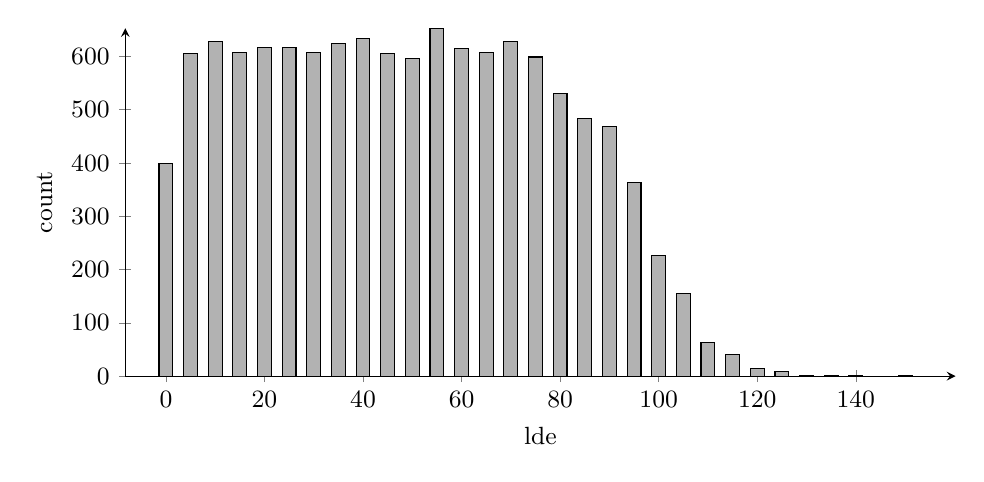
\begin{tikzpicture}
    \begin{axis}[
                    ybar=0pt,
                    bar width=5pt,
                    width=\linewidth,
                    height=6cm,
                    xlabel={lde},
                    ylabel={count},
                    ymin=0,
                    xmin=-5, xmax=157,
                    xtick={0,20,40,60,80,100,120,140},
                    ytick={0,100,200,300,400,500,600},
                    tick label style={font=\small},
                    label style={font=\small},
                    axis lines=left,
                    enlarge x limits=0.02,
            ]
            \addplot[fill=black!30, draw=black] coordinates {
                            (0,399) (5,606) (10,628) (15,608) (20,617) (25,616) (30,607)
                            (35,624) (40,634) (45,605) (50,596) (55,653) (60,615) (65,608)
                            (70,628) (75,599) (80,530) (85,483) (90,468) (95,364) (100,226)
                            (105,155) (110,63) (115,40) (120,14) (125,9) (130,2) (135,1)
                            (140,1) (150,1)
                    };
         \end{axis}
  \end{tikzpicture}
  \caption{Distribution of the least denominator exponent (lde) across
    the 12{,}000 test operators, binned in groups of 5. The lde ranges
    from 0 to 152, with a mean of 51 and a median of 50.}
  \label{fig:lde-dist}
\end{figure}


% Figure 2: K-count reduction distribution (2% bins)
\begin{figure}
  \centering
  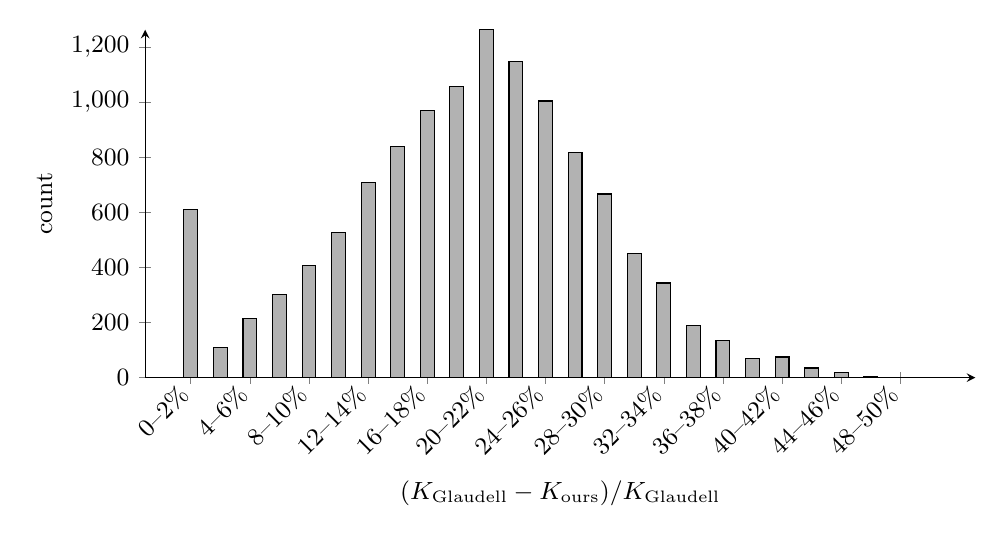
\begin{tikzpicture}
    \begin{axis}[
                    ybar=0pt,
                    bar width=5pt,
                    width=\linewidth,
                    height=6cm,
                    xlabel={$(K_{\mathrm{Glaudell}} - K_{\mathrm{ours}}) / K_{\mathrm{Glaudell}}$},
                    ylabel={count},
                    ymin=0,
                    xmin=-1, xmax=53,
                    xtick={1,5,9,13,17,21,25,29,33,37,41,45,49},
                    xticklabels={0--2\%,4--6\%,8--10\%,12--14\%,16--18\%,20--22\%,24--26\%,28--30\%,32--34\%,36--38\%,40--42\%,44--46\%,48--50\%},
                    x tick label style={font=\small, rotate=45, anchor=east},
                    ytick={0,200,400,600,800,1000,1200},
                    tick label style={font=\small},
                    label style={font=\small},
                    axis lines=left,
                    enlarge x limits=0.02,
            ]
            \addplot[fill=black!30, draw=black] coordinates {
                            (1,611) (3,111) (5,214) (7,302) (9,407) (11,527) (13,710)
                            (15,840) (17,970) (19,1058) (21,1264) (23,1148) (25,1005)
                            (27,819) (29,667) (31,451) (33,344) (35,191) (37,135) (39,71)
                            (41,75) (43,35) (45,19) (47,5) (49,1) (51,1)
                    };
    \end{axis}
  \end{tikzpicture}
  \caption{Distribution of the relative $K$-count reduction
    $(K_{\mathrm{Glaudell}} - K_{\mathrm{ours}}) /
    K_{\mathrm{Glaudell}}$, binned in 2\,\% increments. Our method
    improves on Glaudell et al.'s $K$-count in 95.1\,\% of cases, with
    a mean reduction of 19.7\,\%, a median of 20.3\,\%, and a maximum
    of 50.0\,\%.}
  \label{fig:k-reduction-dist}
\end{figure}

The two algorithms produced identical $\CS$-counts on every operator
in the test set, so our algorithm is also $\CS$-optimal in practice.
Our $K$-count is strictly smaller than Glaudell et al.'s in $95.1\,\%$
of cases (Figure~\ref{fig:k-reduction-dist}).


\subsection{Source of improvement}
The data show that Glaudell et al.'s $K$-count is well approximated by
twice the $\CS$-count,
\[
  K_{\mathrm{Glaudell}} \approx 2 \cdot \mathit{CS}\text{-count},
\]
and, consistent with Lemma~\ref{lem:prkc}, that our $K$-count is well
approximated by twice the lde,
\[
  K_{\mathrm{ours}} \approx 2 \cdot \mathrm{lde}.
\]
The absolute $K$-count saving is therefore approximately
$2 \cdot (\mathit{CS}\text{-count} - \mathrm{lde})$. The relative
reduction is roughly stable across lde values, hovering around
$19$--$21\,\%$ for lde between $5$ and $80$ and tapering off at the
extremes (possibly due to smaller sample sizes).

\subsection{Worst cases}
For $588$ of the $12{,}000$ operators ($4.9\,\%$), our method achieves
no $K$-count reduction (Figure~\ref{fig:k-reduction-dist}). The family
$W_n = (\CK \cdot \KC)^n$ is one of the worst cases: a direct
computation gives $\lde(W_n) = \cs(W_n)$, and on this family our
algorithm and Glaudell et al.'s produce the same $K$-count,
$2 \cdot \lde(W_n)$.

\subsection{Code and data availability}
\label{sec:code}

Code and data are available at \cite{Bian_Kopt}.

\section{Conclusion and future work}

We have presented an efficient, K-optimal, CS-near-optimal algorithm
for the exact synthesis of two-qubit Clifford+$\CS$ circuits from a
given unitary matrix. The theoretical worst-case CS-count is twice
optimal, but in practice our method always achieves the optimal
CS-count and consistently produces a smaller $K$-count than the best
previously known algorithm.

Several directions remain open. The algorithm of Li et al.\
\cite{Li_2023_CT2} produces circuits with $T$-count at most $10$ times
optimal in the worst case; we believe our method can be adapted to
tighten this bound. Total gate count is another natural target, since
experiments show that the raw length of our output is well below the
theoretical bound. Extending to the three-qubit case is plausible,
though the number of residue patterns is likely far greater than the
six in Lemma~\ref{lem:main}, which may complicate the analysis and
weaken the bounds; the four-qubit case is harder still. Extending to
the two-qubit Clifford+V and Clifford+Cyclotomic gate sets is a
promising avenue. Finally, since our method achieved CS-optimality on
all $12{,}000$ randomly generated test operators, we conjecture that
it is in fact CS-optimal, and we leave the proof to future work.

\section{Acknowledgments}
The authors acknowledge support from the National Natural Science
Foundation of China under Grant 92465202. Claude Opus 4.6 was used to
improve the wording of the paper, generate the distribution diagrams
(Figures~\ref{fig:lde-dist} and~\ref{fig:k-reduction-dist}), and draft
initial versions of the Haskell file \texttt{Glaudell.hs}. All
AI-generated content was verified by the authors.

%------------------------------------------------
\bibliographystyle{abbrv}
\bibliography{thesis}

\end{document}
